\documentclass{exam-zh}
\usepackage{siunitx}
\usepackage[version=4]{mhchem}
\usepackage{pifont}
\usepackage{xfrac}
\usepackage{CJKfntef}
\usepackage{vbbool}

\usepackage{makecell,multirow,diagbox}

\newcommand{\lud}[1]{\CJKunderdot{#1}}
\newcommand{\lunl}[1]{\underline{\hbox to #1{}}}%%  可输入长度的下划线
\newcommand{\lminiindent}[1]{\makebox[-1em]{#1\qquad}} % 缩进
\newcommand{\rmnum}[1]{\romannumeral #1} % 小写罗马数字
\newcommand{\Rmnum}[1]{\uppercase\expandafter{\romannumeral #1\relax}} % 大写罗马数字

\usetikzlibrary{
  arrows,
  fit,
  intersections,
  quotes,
  angles,
	positioning,
	mindmap,
	shadows,
	backgrounds,
	math,
	calc,
	decorations.markings,
	decorations.pathmorphing,
  decorations.text,
	patterns
	}

\examsetup{
  page/size=a4paper,
  paren/show-paren=true,
  paren/show-answer=false,
  fillin/show-answer=false,
  %solution/show-solution=show-move
}
\ExamPrintAnswerSet{
	paren/show-paren=false,
}


\everymath{\displaystyle}

\title{26河南高考}

\subject{物理}



\begin{document}

% \information{
%   姓名\underline{\hspace{6em}},
%   座位号\underline{\hspace{15em}}
% }
% \warning{（在此卷上答题无效）}

\secret

\maketitle
  本试卷共6页，15题。全卷满分100分。考试用时75分钟。

\begin{notice}
  \item 答题前，先将自己的姓名、准考证号、考场号、座位号填写在试卷和答题卡上，并将准考证号条形码粘贴在答题卡上的指定位置。
  \item 选择题的作答：每小题选出答案后，用 2B 铅笔把答题卡上对应题目的答案标号涂黑。写在试卷、草稿纸和答题卡上的非答题区域均无效。
  \item 填空题和解答题的作答：用黑色签字笔直接答在答题卡上对应的答题区域内。写在试卷、草稿纸和答题卡上的非答题区域均无效。
  \item 考试结束后，请将本试卷和答题卡一并上交。
\end{notice}

\section{%
	单项选择题：本题共7小题，每小题4分，共28分。在每小题给出的四个选项中，只有一项符合题目要求。}
\begin{question}
	\icode{N26Y-MG-SI-L2-260626-001}
\nceeID[4]{2026河南}{1}
将一单摆的摆球拉开一个小角度后释放，单摆摆动的振幅为 \(A_{0}\)，周期为 \(T_{0}\)。若将此摆移到月球上，拉开相同的角度，则摆球的振动图像可能正确的是\paren[]

\begin{choices}
\item 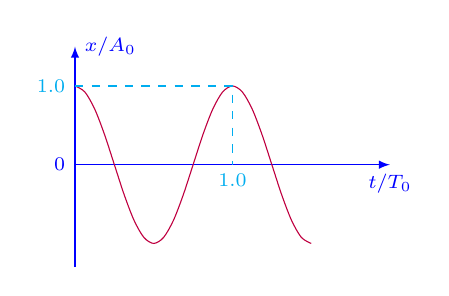
\begin{tikzpicture}[>=latex,font=\scriptsize]
    \draw[->,blue] (0,-1.3)--(0,1.5)node[right]{\(x\)/\(A_0\)};
    \draw[->,blue] (0,0)node[left]{0}--(4,0)node[below]{\(t\)/\(T_0\)};
    \draw[purple,domain=0:3,smooth] plot(\x,{cos(pi*\x r)});
    \draw[dashed,cyan] (0,1)node[left]{1.0}--(2,1)--(2,0)node[below]{1.0};
    \end{tikzpicture}
\item 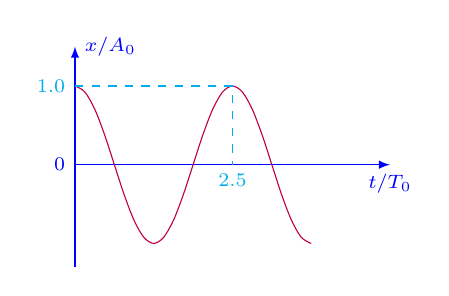
\begin{tikzpicture}[>=latex,font=\scriptsize]
    \draw[->,blue] (0,-1.3)--(0,1.5)node[right]{\(x\)/\(A_0\)};
    \draw[->,blue] (0,0)node[left]{0}--(4,0)node[below]{\(t\)/\(T_0\)};
    \draw[purple,domain=0:3,smooth] plot(\x,{cos(pi*\x r)});
    \draw[dashed,cyan] (0,1)node[left]{1.0}--(2,1)--(2,0)node[below]{2.5};
    \end{tikzpicture}
\item 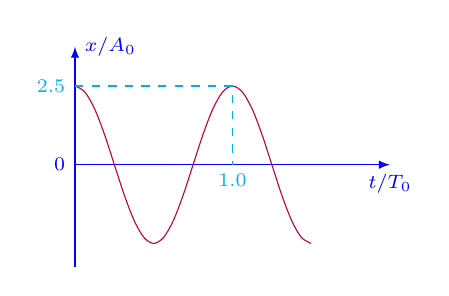
\begin{tikzpicture}[>=latex,font=\scriptsize]
    \draw[->,blue] (0,-1.3)--(0,1.5)node[right]{\(x\)/\(A_0\)};
    \draw[->,blue] (0,0)node[left]{0}--(4,0)node[below]{\(t\)/\(T_0\)};
    \draw[purple,domain=0:3,smooth] plot(\x,{cos(pi*\x r)});
    \draw[dashed,cyan] (0,1)node[left]{2.5}--(2,1)--(2,0)node[below]{1.0};
    \end{tikzpicture}
\item 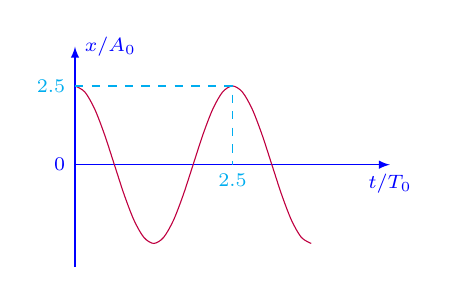
\begin{tikzpicture}[>=latex,font=\scriptsize]
    \draw[->,blue] (0,-1.3)--(0,1.5)node[right]{\(x\)/\(A_0\)};
    \draw[->,blue] (0,0)node[left]{0}--(4,0)node[below]{\(t\)/\(T_0\)};
    \draw[purple,domain=0:3,smooth] plot(\x,{cos(pi*\x r)});
    \draw[dashed,cyan] (0,1)node[left]{2.5}--(2,1)--(2,0)node[below]{2.5};
    \end{tikzpicture}
\end{choices}
\begin{answer}
    B\quad 提示：单摆周期公式\(T = 2\pi \sqrt{\frac{l}{g}}\)，月球重力加速度约为地球的\(\frac{1}{6}\)，\(\sqrt{6} = \sqrt{2}\cdot\sqrt{3} =2.45\)
\end{answer}
\end{question}


\section{%
	多项选择题:本题共3小题，每小题6分,共18分。在每小题给出的选项中，有多项符合题目要求，全部选对的得6分，选对但不全的得3分，有选错的得0分。}



\section{%
		非选择题：本题共5小题，共54分}
	

\end{document}